\input{header.tex}

\begin{document}

\title{{\sc Lycoris}{\bf : A large area beam telescope based on hybrid-less strip silicon sensors}}
\author[3]{Martin Breidenbach}
\author[3]{Dietrich R. Freytag}
\author[1]{Uwe Kraemer}
\author[3]{Benjamin A. Reese}
\author[2,1]{Sebastiaan Roelofs}
\author[1]{Marcel Stanitzki}
\author[1]{Mengqing Wu}
\affil[1]{\footnotesize Deutsches Elektronen-Synchrotron DESY, Notkestr. 85, 22607 Hamburg, Germany}
\affil[2]{\footnotesize The Hague University of Applied Sciences, Rotterdamseweg 137, 2628 AL Delft, The Netherlands}
\affil[3]{\footnotesize Stanford Linear Accelerator Center SLAC, 2575 Sand Hill Road, Menlo Park, CA 94025 USA}
\maketitle

\begin{abstract}
%\linenumbers

A new Large area x-Y COverage Readout Integrated Strip telescope (\lycoris) is being constructed
as an improvement of the DESY test beam infrastructure within the Horizon2020 AIDA-2020 project~\cite{aida2020}.
The \lycoris telescope consists of six layers of \SI{25}{\micro\metre} pitch strip Si sensor readout by two bump-bonded ASICs (KPiX),
running at a timing resolution as multiples of \SI{80}{\nano\second};
its active area is designed to be 10$\times$\SI{10}{\square\centi\metre}, extendable to 10$\times$\SI{20}{\square\centi\metre}.
It can run either standalone or be mounted inside a \SI{1}{\tesla} solenoid magnet,
providing a spatial resolution better than \SI{10}{\micro\metre} along the bending direction,
and a resolution better than \SI{1}{\milli\metre} along the magnetic field.
The full readout system was tested with a hexagonal pixel sensor designed for the SiD ECAL in the lab with a $^{90}$Sr source,
and later tested in the electron beam at DESY in May and October 2017. The first assembled modules with the final strip were tested in spring 2018.
First results of the \lycoris prototype will be presented with a comparison to simulation,
besides, the characterization of sensor and readout system are also included.
\end{abstract}

\section*{Motivation and Concept}
%\linenumbers

The DESY II Test Beam Facility\cite{desytbf} provides $e^-/e^+$ beams with energies from 1 to \SI{6}{\GeV} up to \SI{1}{\MHz}
%converted from bremsstrahlung beams from carbon fibre targets in the electron-positron synchrotron DESY II,
with three test beam lines (TB21, TB22 and TB24).
The beam lines TB21 and TB22 are both equipped with a EUDET-type beam telescope~\cite{eudet} with an active area of around 1$\times$\SI{2}{\square\centi\metre},
which is based on a fine pitch \uppercase{mimosa}~26 monolithic sensor with an event readout frame of \SI{115.2}{\micro\second};
the beam line TB24 is equipped with a \SI{1}{\tesla} solenoid, the PCMAG, at a diametre of $\sim$\SI{85}{\centi\metre} with its wall of $\sim20X_0$,
inside which both the EUDET-type telescope and the Device Under Test (DUT) can be inserted.
The EUDET-type beam telescopes at DESY are proven to meet user demands very well and thus in a high ($\sim$70\%) demand,
however, its active area is limited for momentum measurements for users in the PCMAG or for users requiring a larger tracker coverage..
Therefore, a new telescope is in need to provide a spatial resolution better than \SI{10}{\micro\metre} along the bending direction,
and a resolution better than \SI{1}{\milli\metre} along the magnetic field,
with a large active area of 10$\times$10/\SI{20}{\square\centi\metre},
to cover 90\% to 96\% of the incoming particles with energies from 1 to \SI{6}{\GeV} considering momentum smearing after the magnet wall.

\begin{figure}[!ht]%
\centering
%\vspace{-10px}
%\hspace{-100px}
%\parbox{1.2in}{
\includegraphics[width=0.49\linewidth]{pics/principle.pdf}
%}%
%\hspace{150px}
%\begin{minipage}{1.2in}%
\includegraphics[width=0.49\linewidth]{pics/sensor_module1.jpg}
%\end{minipage}%
\caption{Left: sketch of the \lycoris telescope, where the black lines symbolize the module connection;
Right: photo of an assembled module with two bump-bonded KPiX chips. The KPix are read out using a kapton-flex cable which is glued onto the sensor and connected to the KPix using wirebonds.}%
\label{fig:1figs}%
\end{figure}

The 10$\times$\SI{10}{\square\centi\metre} SiD tracker strip sensor at a pitch of \SI{25}{\micro\metre}, readout by two 1024-channel ASICs, KPiX~\cite{kpix}, can provide a resolution of around \SI{7.2}{\micro\metre},
was hence chosen, and the other requirements can be achieved by a \SI{2}{\degree} tilt. This sensor was originally developed for the SiD Detector Concept for the ILC~\cite{Behnke:2013lya}.
The new telescope, \lycoris is finally designed as a 6-plane strip telescope in a mirror symmetric setup, with its upstream orientation of (0, -\SI{2}{\degree}, \SI{2}{\degree}),
see Figure~\ref{fig:1figs} (left), and it is controlled by a custom FPGA board.
When a beam particle passes a Photomultiplier (PMT), the connected Trigger Logic Unit (TLU) will send a trigger to the telescope and to the DUT for synchronization;
the telescope data is digitized and readout by the bump-bonded KPiXs, then packed by the DAQ board and sent to the connected PC. A common DAQ software from the beam telescope
community, EUDAQ2~\cite{eudaq2}, is used, which helps to synchronize the run control of telescope, TLU, and DUT. It also greatly simplifies the integration of user DAQ systems.

\section*{Assembly and Tests}

The KPiX readout system was characterized before the final strip sensor delivery with several hexagonal pixel sensors, whic  were originally designed for the SiD ECAL~\cite{Behnke:2013lya}
and are using the KPiX as well. These tests included understanding how to synchronize the KPiX chip data taking cycles to the DESY beam structure, as well as to other devices, like the TLU, and various DUTs.
It was tested first with a $^{90}$Sr source in the lab, and then in the DESY test beam with energies from 4 to \SI{6}{\GeV} in May and October 2017~\cite{lycoris1}.

The strip sensors were delivered by Hamamatsu in summer 2017, showing very good electric features and all fully depleted at around \SI{50}{\volt}.
The first assembled sensors, see one example in Figure~\ref{fig:1figs} (right), were tested in spring 2018, with a $^{90}$Sr source in the lab at DESY, and several DESY test beam weeks are in schedule in fall 2018.
Figure~\ref{fig:2figs} shows the fired strip distribution over one data taking run, collected by one KPiX chip in a self-trigger mode from one assembled module, using a $^{90}$Sr source ,
demonstrating that the assembled module is capable of seeing signals.

\begin{figure}[!ht]%
\centering
%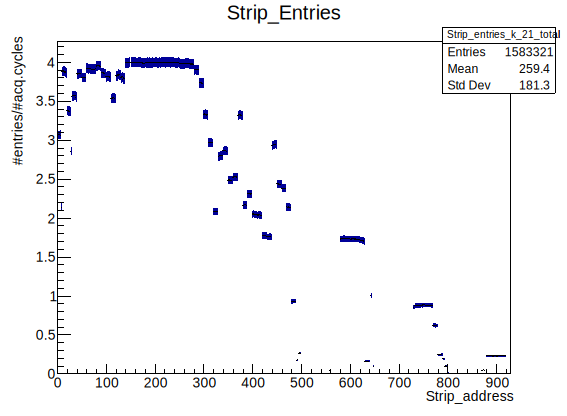
\includegraphics[width=0.49\linewidth]{pics/S58_K2_2018_05_07_16_49_42_strip_entries.png}
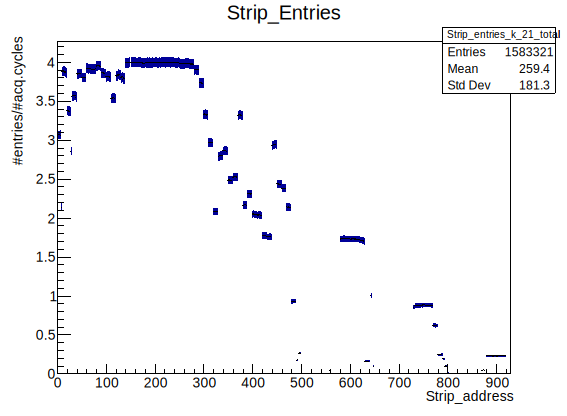
\includegraphics[width=0.46\linewidth]{pics/S58_K2_2018_05_07_16_49_42_strip_entries.png}
\caption{The fired strip distribution over one assembled module, data collected from one KPiX in a self-trigger mode under a $^{90}$Sr source. }%
\label{fig:2figs}%
\end{figure}

The \lycoris telescope is scheduled to be delivered early 2019, with a TLU and a reconstruction software ready-to-use for user.
In this contribution, the \lycoris telescope will be presented, with its first results and a comparison to simulation;
the characterization of the sensor and readout system will also be included.

\footnotesize
\begin{thebibliography}{1}
\bibitem{aida2020} AIDA2020 homepage \url{http://aida2020.web.cern.ch}, Accessed on 2018-04-05
\bibitem{desytbf} DESY II Test Beam Facility \url{http://testbeam.desy.de}, Accessed on 2018-04-05
\bibitem{eudet} H.~Jansen et al., {\em Performance of the EUDET-type beam telescopes},
\textbf{EPJ Tech.\ Instrum.\  {\bf 3}, no. 1, 7 (2016)}.

\bibitem{kpix} J.~Brau et al., {\em KPiX - A 1,024 channel readout ASIC for the ILC},
\textbf{in 2012 IEEE Nuclear Science Symposium and Medical Imaging Conference Record (NSS/MIC), pp. 1857–1860, Oct 2012.}.
\bibitem{Behnke:2013lya}  T.~Behnke et al.,{\em The International Linear Collider Technical Design Report - Volume 4: Detectors}
\textbf{  arXiv:1306.6329 [physics.ins-det]}
\bibitem{eudaq2} Y.~Liu., {\em EUDAQ2 User Manual},
\textbf{AIDA-2020-NOTE-2018-001}.

\bibitem{lycoris1} U.~Kraemer et al., {\em LYCORIS - A Large Area Strip Telescope},
\textbf{arXiv:1801.08505 [physics.ins-det]}.


\end{thebibliography}

\end{document}
